\documentclass[a4paper,12pt]{memoir}

\usepackage{fontspec}
\usepackage[margin=2.5cm]{geometry}
\usepackage{enumitem}

\makeevenfoot{headings}{}{\thepage}{}
\makeoddfoot{headings}{}{\thepage}{}
\makeevenhead{headings}{37-2431-D/PCC/unofficial}{}{}
\makeoddhead{headings}{}{}{37-2431-D/PCC/unofficial}

\setlist[description]{labelindent=1em, listparindent=5em}

\newcommand{\sign}[2]{%
\noindent\makebox[\linewidth][c]{%
    \begin{minipage}{0.4\linewidth}
    \hrulefill\par
    \centering
    #1\par#2
  \end{minipage}}
}

\makeatletter
\newcommand{\checkitem}[2][,]{%
   \item[#2]\hfill \begin{description}\checknextarg}
\newcommand{\checknextarg}{\@ifnextchar\bgroup{\gobblenext}{}}% Check if another "argument" exists
\newcommand{\gobblenext}[1]{\item {#1}\@ifnextchar\bgroup{\gobblenext}{\end{description}}}% Gobble next "argument"
\makeatother

\newcommand{\button}[1]{\makebox[5.5em][l]{■ #1}}
\newcommand{\knob}[1]{\makebox[5.5em][l]{◊ #1}}
\newcommand{\lamp}[1]{\makebox[5.5em][l]{☼ #1}}
\newcommand{\switch}[1]{\makebox[5.5em][l]{♦ #1}}
\newcommand{\nowt}{\makebox[5.5em][l]{}}

\setmainfont{Noto Sans}

\begin{document}
{\Huge{\fontspec{Michroma}FLIGHT DATA FILE}
\par\vspace{3ex}
\textbf{Prelaunch Cockpit Checklist}\par
\par\vspace{3ex}
\textbf{37-2431-D \textit{FireArc}}
\par\hrulefill
\par\vspace{5ex}
}
{\LARGE \textbf{Flight Design and Dynamics Division}
\par
\textbf{Unofficial}
\par
\textbf{13 July, 3300}
}

\begin{picture}(50,340) \put(280,0){\hbox{\includegraphics[scale=0.3]{RogSys_LOGO1024}}} \end{picture}
\newpage
\begin{center}\begin{vplace}This page intentionally blank\end{vplace}\end{center}
\newpage
\begin{center}
VEHICLE OPERATIONS DIRECTORATE
\par\vspace{2ex}
\textbf{PRELAUNCH COCKPIT CHECKLIST}
\par
\textbf{37-2431-D}
\par\vspace{2ex}
DRAFT
\par
13 July, 3300
\par\vspace{2ex}
PREPARED BY:
\par\vspace{8ex}
\sign{John Dee}{Book Manager}
\par\vspace{6ex}
APPROVED BY:
\par\vspace{8ex}
\sign{Michael Juliano}{Project Director}
\end{center}
\newpage
\begin{figure}[!h]
\centering
\includegraphics[width=0.8\textwidth]{left_panel.pdf}
\caption{Left-side instrument panel}
\end{figure}
\newpage
\begin{figure}[!h]
\centering
\includegraphics[width=0.8\textwidth]{right_panel.pdf}
\caption{Right-side instrument panel}
\end{figure}
\newpage
\begin{center}\begin{vplace}This page intentionally blank\end{vplace}\end{center}
\newpage
\begin{center}\begin{vplace}\underline{PRESTART PROCEDURES}\end{vplace}\end{center}
\newpage
\noindent\makebox[\linewidth][c]{%
\begin{minipage}{0.7\linewidth}
\textbf{PRESTART PROCEDURES}

\begin{description}
\checkitem{SEAT SAFING}%
{\button{CSSM}SEAT SAFE — ON}

\checkitem{LIGHTING}%
{\button{CSSM}CABIN FLOOD LIGHT — OFF}%
{\button{CSSM}INST LIGHT — ON}

\checkitem{PRIMARY BUS POWER}%
{\knob{BATT}SELECT set to SYS1}%
{\button{BATT}POWER — ON}%
{\knob{ECS}BUS SELECT set to PRI}%
{\button{ECS}POWER — ON}%
{…Wait 4 sec for fault alarm, then…}%
{\button{HMD}FAULT ACK — PRESS}

\checkitem{BATTERY CHARGE}%
{\button{ECS}MAINT CUT-OFF — OFF}%
{\button{BATT}RECHARGE — ON}%
{\knob{BATT}SELECT set to SYS2}%
{\button{BATT}POWER — ON}%
{\button{BATT}RECHARGE — ON}

\checkitem{SECONDARY BUS POWER}%
{\knob{ECS}BUS SELECT set to SEC}%
{\button{ECS}POWER — ON}%
{\knob{ECS}DISTRIBUTION MODE set to BAL}

\checkitem{FUEL CELL CHARGE}%
{\knob{FCS}CELL SELECT set to SYS1}%
{\button{FCS}POWER — ON}%
{…wait for CORE TEMP rise to start, then…}%
{\knob{FCS}CELL SELECT set to SYS2}%
{\button{FCS}POWER — ON}%
{…wait for CORE TEMP rise to start}

\end{description}
\end{minipage}}
\newpage
\noindent\makebox[\linewidth][c]{%
\begin{minipage}{0.7\linewidth}
\begin{description}

\checkitem{THERMAL MANAGEMENT}%
{\button{TMS}LOOP ENABLE — ON}%
{\knob{TMS}LOOP SELECT set to SYS1}%
{\button{TMS}LOOP PRESSURIZE — ON}%
{\switch{TMS}LOOP PUMP POWER set to ON}%
{\knob{TMS}LOOP SELECT set to SYS2}%
{\button{TMS}LOOP PRESSURIZE — ON}%
{\switch{TMS}LOOP PUMP POWER set to ON}

\checkitem{STC DEPARTURE CLEARANCE}%
{\button{COMMS}SYSTEM ENABLE — ON}%
{\button{COMMS}TRANSMITTER ENABLE — ON}%
{Check in with STC}%
{…wait for STC check in acknowledge, then…}%
{Request departure clearance from STC}%
{…wait for STC departure clearance}

\end{description}
\end{minipage}}

\newpage
\begin{center}\begin{vplace}This page intentionally blank\end{vplace}\end{center}
\newpage
\begin{center}\begin{vplace}\underline{DEPARTURE PROCEDURES}\end{vplace}\end{center}
\newpage
\noindent\makebox[\linewidth][c]{%
\begin{minipage}{0.7\linewidth}
\textbf{DEPARTURE PROCEDURES}

\begin{description}
\checkitem{ENGINE INITIALISE}%
{\knob{MES}ENGINE SELECT set to ENG1}%
{\button{MES}SYSTEM ENABLE — ON}%
{\button{MES}LENR ENABLE — ON}%
{\button{MES}CHAMBER PRE-HEATER — ON}%
{\button{RCM}SYSTEM ENABLE — ON}%
{\button{RCM}ENABLE ALL TANKS — ON}%
{\button{MES}FUEL SOURCE SELECT — ON}%
{\knob{FCS}CELL SELECT set to SYS1}%
{\button{FCS}FUEL SOURCE SELECT — ON}%
{\button{FCS}REACTANT SOURCE SELECT — ON}%
{\knob{FCS}CELL SELECT set to SYS2}%
{\button{FCS}FUEL SOURCE SELECT — ON}%
{\button{FCS}REACTANT SOURCE SELECT — ON}%
{Request LENR initiation from STC}%
{…wait for STC LENR initiation clearance}

\checkitem{MAIN BUS INITIALISE}%
{\button{MES}LENR FUEL CUT-OFF — ON}%
{\button{MES}LENR FUSE ENABLE - ON}%
{\knob{ECS}BUS SELECT set to MAIN}%
{\button{ECS}POWER — ON}%
{\button{ECS}MAINT CUT-OFF — ON}

\checkitem{MTS COLD GAS INITIALISE}%
{\button{MTS}SYSTEM ENABLE — ON}%
{\button{MTS}FUEL SOURCE SELECT — ON}%
{\button{MTS}FUEL CUT-OFF VALVE — ON}%
{\button{MTS}FUEL INJECTOR ENABLE — ON}%
{\button{MTS}NOZZLE ALL ENABLE — ON}

\checkitem{NAVIGATION INITIALISE}%
{\button{NAS}SYSTEM ENABLE — ON}

\end{description}
\end{minipage}}
\newpage
\noindent\makebox[\linewidth][c]{%
\begin{minipage}{0.7\linewidth}
\begin{description}

\checkitem{SEAT SAFING}%
{\knob{CSSM}FLIGHT MODE SELECT set to NORM FLIGHT}
{Announce to STC ready to depart}
\end{description}
\end{minipage}}

\end{document}
